\documentclass[utf8]{article}
\usepackage{graphicx} % Required for inserting images
\usepackage[utf8]{inputenc}
\usepackage{float}

\title{AD Aufgabe 3 Dokumentation}
\author{Anton Tchekov, Haron Nazari\\ Praktikums Gruppe 3, Team 2}
\date{December 2023}

\begin{document}
\maketitle

\section{Abstract}
In dieser Dokumentation geht es um verschiedene Datenstrukturen an denen
Algorithmen angewendet wurden.
Die Datenstrukturen umfassen Binary Trees, Binary Search Trees und Graphen.
Wir haben bei dem Graphen die Laufzeit der Suchalgorithmen getestet und
beim Binary Search Tree die durchschnittliche Pfadlänge bestimmt.

// TODO ergebnis

\section{Einführung}
Die angewendeten Algorithmen für den Graphen umfassen:
\begin{enumerate}
  \item Tiefensuche
  \item Breitensuche
  \item Kürzeste Pfade nach Dijkstra
\end{enumerate}
Für den Binary Seach Tree wurde nur die durschnittliche Pfadlänge für
unterschiedliche Baumgrößen von n = 100 bis n = 10 000 (in 100er Schritten)
berechnet und in einem Graphen geplottet und mit der
Funktion \emph{1.39 * log2(x) - 1.85} verglichen.
\pagebreak
\section{Dokumentation}

\subsection{Beschreibung von Verfahren/Implementation}

\paragraph{Graphen}
Der Graph wurde mit Adjazenzlisten implementiert

\begin{verbatim}
public class Vertex<E>
{
  private E content;
  private HashMap<Vertex<E>, Integer> neighbours;

  [...]
}
\end{verbatim}
Jeder Knoten hat eine Liste von seinen Nachbarn, inklusive des
Gewichts der Kante zu dem jeweiligen Nachbarn.\\\\
\textbf{Breitensuche} \label{Breitensuche}
Die Breitensuche wurde mithilfe einer Queue implementiert.
Man ereiht den Startknoten ein und überprüft ob dieser das Ziel ist,
falls nicht, werden alle Nachbarn in die Queue gepackt und nacheinander
wie der Startknoten abgesucht. Falls man das Element findet beendet sich der Suchalgorithmus\\
\\
\textbf{Tiefensuche}
Die Tiefensuche wurde wie die Breitensuche implementiert jedoch wurde
statt einer Queue ein Stack verwendet. \\
\\
\textbf{Dijkstra}
\paragraph{1.}
Beim Dijkstra wird eine Priority Queue verwendet, die aufsteigend nach
der Summe des Gewichtes sortiert ist.
Es wird zuerst das Startelement in die Queue eingereiht,
mit den Parametern: Kein vorheriger Knoten,
der zugehörige Knoten und das Gesamtgewicht bis zu diesem Knoten.
\paragraph{2.} Es wird dann aus der Queue ein Element genommen, falls dieses nicht das gesuchte
Element ist, wird von dem genommenen Element alle Nachbarn mit folgenden
Parametern eingereiht: Das jetzige Element, Der jeweilige Nachbarknoten
und die Summe des Gewichtes bis zum jetzigen Knoten. Es wird das Element mit der kleinsten Summe
aus der Liste genommen und Schritt 2 wird wiederholt bis das Element
gefunden wurde. Es wird anschließend der Pfad zurückgegeben.

\subsection{Validierung und Tests}
\paragraph{Dijkstra Algorithmus Laufzeit Testung}
Die Laufzeit vom Dijkstra Algorithmus wurde mit 3 Verschiedenen Szenarien getestet
\begin{enumerate}
  \item Ein Worst-case Szenario. in welchem ein quadratischer Graph, der aufgebaut ist
  wie ein Schachfeld. Ganz unten links wurde der Startpunkt gesetzt und
  ganz oben rechts der Endpunkt, zudem haben alle Kanten die Gewichtung 1.
  Das führt dazu das der Dijkstra jeden Knoten besucht bevor es den Zielknoten
  erreicht. Die Laufzeit wurde dabei geplottet. Siehe Figur 1.

  \begin{figure}[H]
    \centering
    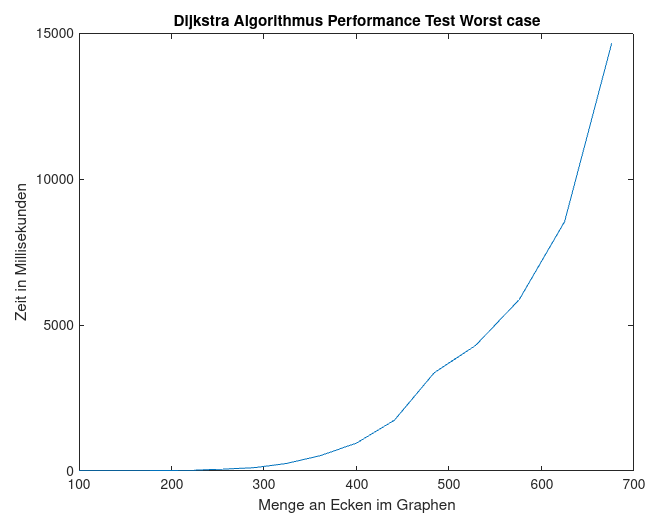
\includegraphics[width=1\textwidth]{Images/Worstcase.png}
    \caption[]{Laufzeit des beschribenen Worst-case Szenarios}
  \end{figure}

  \item Ein Average-Worst-case Szenario, in welchem das gleiche Szenario wie
  1. herrscht, jedoch hat jede Kante eine zufällige Gewichtung von 0-10.
  Für jeden Messpunkt wurde 3 mal getestet. Die Laufzeit wurde auch hier geplottet.
  Siehe Figur 2.

  \begin{figure}[H]
    \centering
    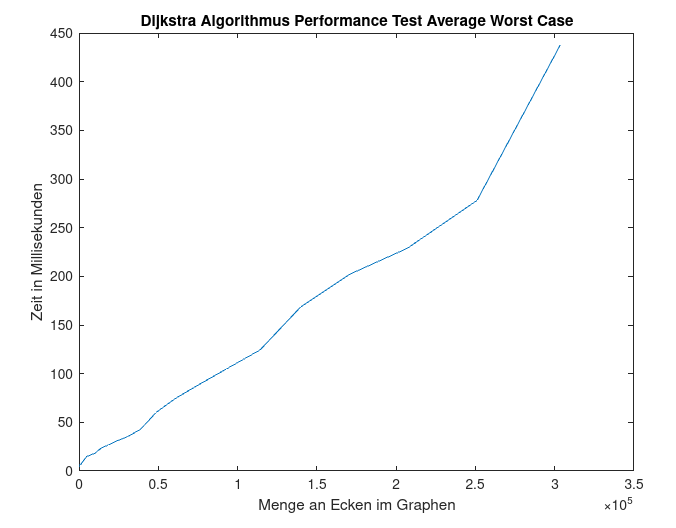
\includegraphics[width=1\textwidth]{Images/AverageWorstCase.png}
    \caption[]{Laufzeit des beschribenen Average-Worst-case Szenarios}
  \end{figure}

  \item Ein Random Non-Dense-case, in welchem ein zufälliger Graph
  auf folgende Weise erstellt wurde: Es wird ein neuer Knoten erstellt und
  mit bis zu 15 von den vorherigen Knoten mit einem zufälligen Gewicht
  zwischen 0 und 15 verbunden. Dies wird dann wiederholt bis die erwünschte Menge
  an Knoten erstellt wurde. Auf diese Weise ist der Graph weniger dicht
  als in den ersten beiden Szenarios. Für jeden Messpunkt wurden
  10 Messungen durchgeführt und das Maximum genommen. Siehe Figur 3.

  \begin{figure}[H]
    \centering
    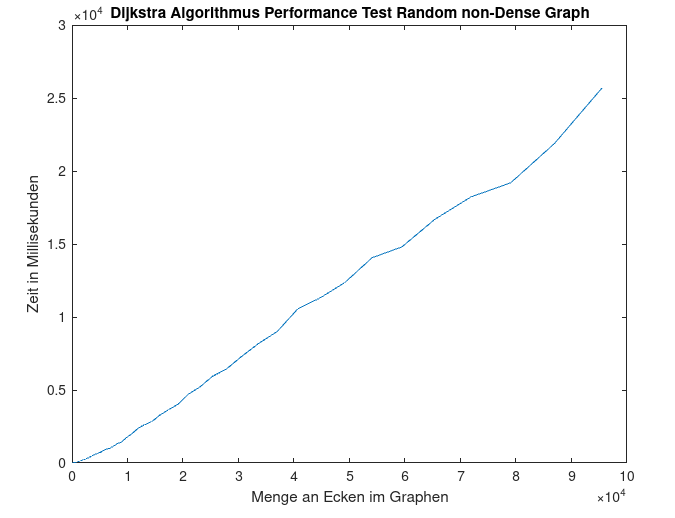
\includegraphics[width=1\textwidth]{Images/Random Non-dense case.png}
    \caption[]{Laufzeit des beschribenen Random Non-Dense-case Szenarios}
  \end{figure}

\end{enumerate}

\paragraph{Fazit Dijkstra} Die Laufzeit von Szenario 1 und 2 richten sich nach
$O(n^2)$, das Szenario 3 jedoch nach $O(n)$. Die Laufzeit ist bei den ersten beiden
Szenarien wie erwartet, beim dritten Szenario scheint der Algorithmus einen
linearen Weg zu finden zum Ziel.

\paragraph{Pfadlaenge des Binary Search Trees}
Um die durchschnittliche Pfadlänge zu bestimmen, haben wir
eine Operation zu dem binären Suchbaum hinzugefügt, welche
ein Element findet und dabei die Anzahl der traversierten
Kanten zählt.\\\\
In einer Schleife werden N zufällig generierte Schlüssel in den Baum
und in eine Liste eingefügt und dann wird für alle Elemente in der
Liste die Pfadlänge bestimmt summiert. Das Resultat der Summe
ist die interne Pfadlänge, die danach durch die Anzahl der Schlüssel
im Baum geteilt wird und um 1 erhöht wird um die durchschnittliche
Pfadlänge zu bestimmen. Für jedes N wird dieser Vorgang 1000 mal
wiederholt und daraus das arithmetische Mittel gebildet um
zufällige Abweichungen auszugleichen.\\\\
Der Ergebnisgraph stimmt mit der angegebenen
Funktion stark überein. Siehe Figur 4.

\begin{figure}[H]
  \centering
  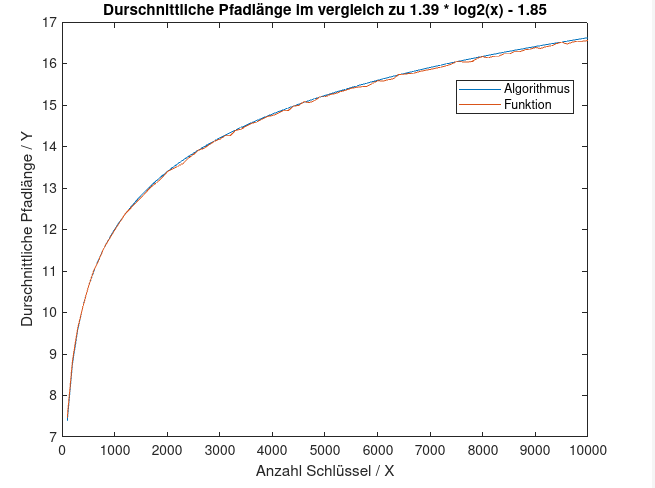
\includegraphics[width=1\textwidth]{Images/Pfadlaenge.png}
  \caption[]{Vergleich zwischen der durschnittlichen Pfadlaenge bei einer
  gegebenen Menge an Schluesselelementen und der Funktion \emph{1.39 * log2(x) - 1.85}}
\end{figure}

\section{Quellen}
Trust me bro.

\end{document}